
\newcommand{\MatrixDiagram}[1]
{    \vspace{0.5cm}
	\begin{figure}[htpb]
		%\hspace{-1.75cm}
		\centering
		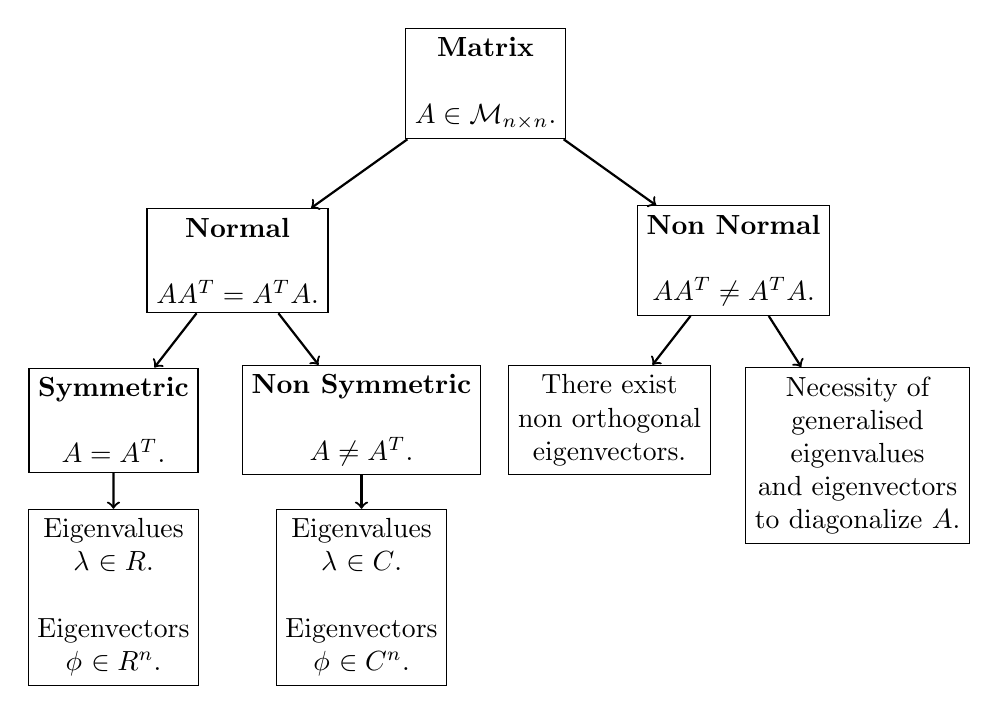
\begin{tikzpicture}[scale=0.9]   	
		
		\tikzstyle{every node}=[draw, align=center, rectangle ]
		
		\node(a) at (0,0) {\textbf{Matrix} \\ \\
			$ A \in \mathcal{M}_{n\times n}.$};
		
		%\node[](b0) at (-7,-2.5) { Normal matrices are \\  diagonalised by \\ orthonormal \\ eigenvectors.};
		
		\node(b1) at (-3.5,-2.5) {\textbf{Normal} \\ \\
			$ A A^T = A^T A.$ };
		
		\node(b2) at (3.5,-2.5) {\textbf{Non Normal} \\ \\
			$ A A^T \neq A^T A.$ };
		
		\node(c1) at (-5.25,-4.75) {\textbf{Symmetric} \\ \\
			$ A = A^T.$  };
		
		\node(c2) at (-1.75,-4.75) {\textbf{Non Symmetric} \\ \\
			$ A \neq A^T.$  };
		
		\node[draw, align=center, rectangle ](c3) at (1.75,-4.75) {There exist\\non orthogonal \\eigenvectors. };
		
		\node(c4) at (5.25,-5.25) {Necessity of \\ generalised \\ eigenvalues\\ and eigenvectors\\ to diagonalize $A$. };
		
		\node(d1) at (-5.25,-7.25) {Eigenvalues \\ $\lambda$ $\in \mathbb{R}$. \\  \\Eigenvectors \\$\phi$ $\in \mathbb{R}^n.$
		};
		
		\node(d2) at (-1.75,-7.25) {Eigenvalues \\ $\lambda$ $\in \mathbb{C}$. \\  \\Eigenvectors \\$\phi$ $\in \mathbb{C}^n.$
		};
		
		\foreach \from/\to in {a/b1, a/b2, b1/c1, b1/c2, b2/c3, b2/c4, c1/d1, c2/d2}
		\draw [->, thick = 1 pt] (\from) -- (\to) ;%node[midway] {\from--\to};
		
		%\draw [->, thick = 1 pt] (a) -- (b) -- (0,-5.25) -- (-2,-5.75) -- (c);
		
		\end{tikzpicture}
		\caption{Normal and non normal matrices classification.}
		\label{fig:MatrixClass}
	\end{figure}
	
}




\newcommand{\nMatrixDiagram}[2]
{    \vspace{0.5cm}
	\begin{figure}[htpb]
		%\hspace{-1.75cm}
		\centering
		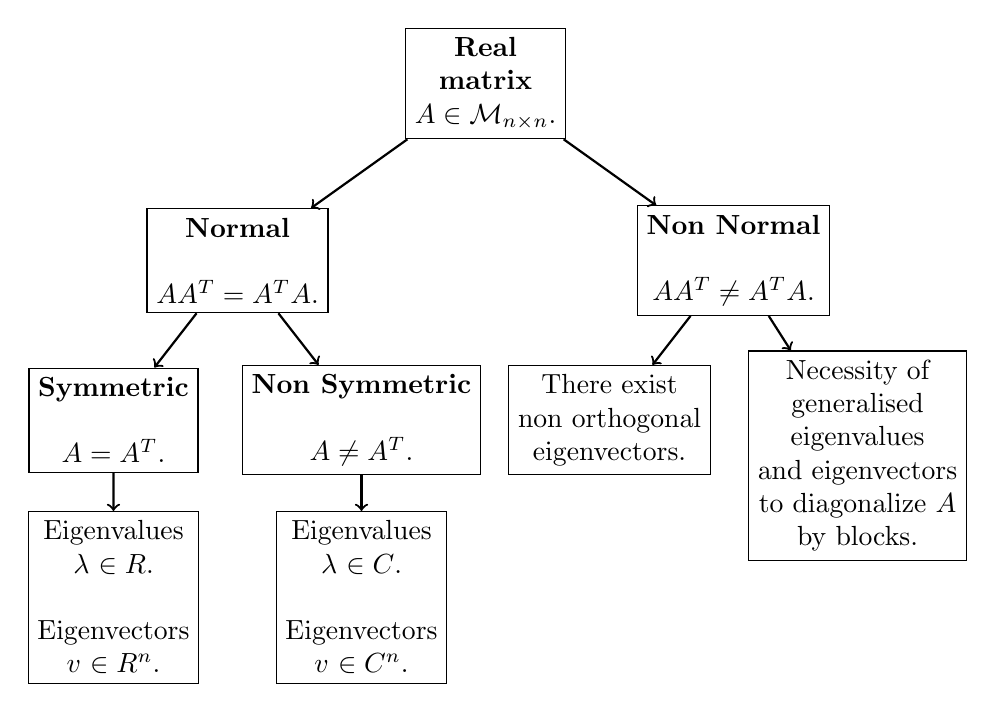
\begin{tikzpicture}[scale=0.9]   	
		
		\tikzstyle{every node}=[draw, align=center, rectangle ]
		
		\node(a) at (0,0) {\textbf{Real} \\\textbf{matrix} \\
			$ A \in \mathcal{M}_{n\times n}.$};
		
		%\node[](b0) at (-7,-2.5) { Normal matrices are \\  diagonalised by \\ orthonormal \\ eigenvectors.};
		
		\node(b1) at (-3.5,-2.5) {\textbf{Normal} \\ \\
			$ A A^T = A^T A.$ };
		
		\node(b2) at (3.5,-2.5) {\textbf{Non Normal} \\ \\
			$ A A^T \neq A^T A.$ };
		
		\node(c1) at (-5.25,-4.75) {\textbf{Symmetric} \\ \\
			$ A = A^T.$  };
		
		\node(c2) at (-1.75,-4.75) {\textbf{Non Symmetric} \\ \\
			$ A \neq A^T.$  };
		
		\node[draw, align=center, rectangle ](c3) at (1.75,-4.75) {There exist\\non orthogonal \\eigenvectors. };
		
		\node(c4) at (5.25,-5.25) {Necessity of \\ generalised \\ eigenvalues\\ and eigenvectors\\ to diagonalize $A$\\  by blocks. };
		
		\node(d1) at (-5.25,-7.25) {Eigenvalues \\ $\lambda$ $\in \mathbb{R}$. \\  \\Eigenvectors \\$\vect{v}$ $\in \mathbb{R}^n.$
		};
		
		\node(d2) at (-1.75,-7.25) {Eigenvalues \\ $\lambda$ $\in \mathbb{C}$. \\  \\Eigenvectors \\$\vect{v}$ $\in \mathbb{C}^n.$
		};
		
		\foreach \from/\to in {a/b1, a/b2, b1/c1, b1/c2, b2/c3, b2/c4, c1/d1, c2/d2}
		\draw [->, thick = 1 pt] (\from) -- (\to) ;%node[midway] {\from--\to};
		
		%\draw [->, thick = 1 pt] (a) -- (b) -- (0,-5.25) -- (-2,-5.75) -- (c);
		
		\end{tikzpicture}
		\caption{#1}
		\label{#2}
	\end{figure}
}


\newcommand{\SVD}[2]
{
\begin{figure}
	\centering
	\begin{tikzpicture}[]
	
\begin{axis}[axis equal image, width = 0.4\textwidth, no marks, axis line style={draw=none}, tick style={draw=none}, xticklabels={,,}, 
yticklabels={,,}]
     \addplot table [skip first n=2, x index=0, y index=1]{./doc/chapters/System_of_Equations/figures/SVD/Geometric/Good_conditioned/x.plt};
     \addplot table [skip first n=2, x index=0, y index=1]{./doc/chapters/System_of_Equations/figures/SVD/Geometric/Good_conditioned/x_v.plt};
     
     \node(Kn) at (0,-0.5) {$\K{n}$};
\end{axis}

\begin{axis}[axis equal image, width = 0.4\textwidth, at={(0.37\linewidth,0)}, no marks, axis line style={draw=none}, tick style={draw=none}, 
xticklabels={,,}, yticklabels={,,}]
	\addplot table [skip first n=2, x index=0, y index=1]{./doc/chapters/System_of_Equations/figures/SVD/Geometric/Good_conditioned/y.plt};
	\addplot table [skip first n=2, x index=0, y index=1]{./doc/chapters/System_of_Equations/figures/SVD/Geometric/Good_conditioned/y_v.plt};
	
	\node(Km) at (0,-0.5) {$\K{m}$};
\end{axis}



\node(x) at (2.5,1.2) {};
\node(A) at (3.5,1.2) {$A$};
\node(y) at (4.5,1.2) {};
\draw[->] (x)--(A)--(y);

\node(x1) at (1.2,0) {};
\node(V) at (1.2,-1) {$V^*$};
\node(v1) at (1.2,-2) {};
\draw[->] (x1)--(V)--(v1);

\node(v2) at (2.5,-3.3) {};
\node(S) at (3.5,-3.3) {$\Sigma$};
\node(s1) at (4.5,-3.3) {};
\draw[->] (v2)--(S)--(s1);

\node(s2) at (5.6,-2) {};
\node(U) at (5.6,-1) {$U$};
\node(y1) at (5.6,0) {};
\draw[->] (s2)--(U)--(y1);

\begin{axis}[axis equal image, width = 0.4\textwidth, at={(0,-0.38\linewidth)}, no marks, axis line style={draw=none}, tick 
style={draw=none}, 
xticklabels={,,}, yticklabels={,,}]
	\addplot table [skip first n=2, x index=0, y index=1]{./doc/chapters/System_of_Equations/figures/SVD/Geometric/Good_conditioned/y1.plt};
	\addplot table [skip first n=2, x index=0, y index=1]{./doc/chapters/System_of_Equations/figures/SVD/Geometric/Good_conditioned/y1_v.plt};
	
	\node(Kn1) at (0,-0.5) {$\K{n}$};
\end{axis}

\begin{axis}[axis equal image,  width = 0.45\textwidth, at={(0.38\linewidth,-0.42\linewidth)}, no marks, axis line style={draw=none}, tick 
style={draw=none}, xticklabels={,,}, yticklabels={,,}]
    \addplot table [skip first n=2, x index=0, y index=1]{./doc/chapters/System_of_Equations/figures/SVD/Geometric/Good_conditioned/y2.plt};
    \addplot table [skip first n=2, x index=0, y index=1]{./doc/chapters/System_of_Equations/figures/SVD/Geometric/Good_conditioned/y2_v.plt};
    
    \node(Km1) at (0,-0.5) {$\K{m}$};
\end{axis}


\end{tikzpicture}
\caption{#1}
\label{#2}
\end{figure}
}




\newcommand{\SVDSingular}[2]
{
	\begin{figure}
		\centering
		\begin{tikzpicture}[]
			
			\begin{axis}[axis equal image, width = 0.4\textwidth, no marks, axis line style={draw=none}, tick style={draw=none}, 
			xticklabels={,,}, yticklabels={,,}]
				\addplot table [skip first n=2, x index=0, y 
				index=1]{./doc/chapters/System_of_Equations/figures/SVD/Geometric/Singular/x.plt};
				
				\node(Kn) at (0,0) {$\K{n}$};
			\end{axis}
			
			\begin{axis}[axis equal image, width = 0.4\textwidth, at={(0.35\linewidth,0)}, no marks, axis line style={draw=none}, tick 
			style={draw=none}, xticklabels={,,}, yticklabels={,,}]
				\addplot table [skip first n=2, x index=0, y 
				index=1]{./doc/chapters/System_of_Equations/figures/SVD/Geometric/Singular/y.plt};
				
				\node(Km) at (-0.5,0) {$\K{m}$};
			\end{axis}
			
			
			
			\node(x) at (2.5,1.2) {};
			\node(A) at (3.5,1.2) {$A$};
			\node(y) at (4.5,1.2) {};
			\draw[->] (x)--(A)--(y);
			
			
			
			
			
		\end{tikzpicture}
		\caption{#1}
		\label{#2}
	\end{figure}
}


\newcommand{\SVDCondition}[2]
{
	\begin{figure}
		\centering
		\begin{tikzpicture}[]
			
			\begin{axis}[axis equal image, width = 0.3\textwidth, no marks, axis line style={draw=none}, tick style={draw=none}, 
			xticklabels={,,}, yticklabels={,,}]
				\addplot table [skip first n=2, x index=0, y 
				index=1]{./doc/chapters/System_of_Equations/figures/SVD/Geometric/Good_conditioned/x.plt};
%				\addplot table [skip first n=2, x index=0, y 
%index=1]{./doc/chapters/System_of_Equations/figures/SVD/Geometric/Good_conditioned/x_v.plt};
				
%				\node(Kn) at (0,-0.5) {$\K{n}$};
			\end{axis}
			
			\begin{axis}[axis equal image, width = 0.3\textwidth, at={(0.3\linewidth,0)}, no marks, axis line style={draw=none}, tick 
			style={draw=none}, xticklabels={,,}, yticklabels={,,}]
				\addplot table [skip first n=2, x index=0, y 
				index=1]{./doc/chapters/System_of_Equations/figures/SVD/Geometric/Good_conditioned/y.plt};
%				\addplot table [skip first n=2, x index=0, y 
%index=1]{./doc/chapters/System_of_Equations/figures/SVD/Geometric/Good_conditioned/y_v.plt};
				
			\end{axis}
			
			
			
			\node(x) at (2.2,1.2) {};
			\node(A) at (3.5,1.2) {$\kappa(A)\sim 1$};
			\node(y) at (5,1.2) {};
			\draw[->] (x)--(A)--(y);
			
			
			
			\node(v2) at (2.2,-2) {};
			\node(S) at (3.5,-2) {$\kappa(A)\gg 1$};
			\node(s1) at (5,-2) {};
			\draw[->] (v2)--(S)--(s1);
			
			
			
			\begin{axis}[axis equal image, width = 0.3\textwidth, at={(0,-0.2\linewidth)}, no marks, axis line style={draw=none}, tick 
			style={draw=none}, xticklabels={,,}, yticklabels={,,}]
				\addplot table [skip first n=2, x index=0, y 
				index=1]{./doc/chapters/System_of_Equations/figures/SVD/Geometric/Bad_conditioned_1/x.plt};
				
			\end{axis}
			
			\begin{axis}[axis equal image,  width = 0.35\textwidth, at={(0.32\linewidth,-0.2\linewidth)}, no marks, axis line 
			style={draw=none}, tick style={draw=none}, xticklabels={,,}, yticklabels={,,}]
				\addplot table [skip first n=2, x index=0, y 
				index=1]{./doc/chapters/System_of_Equations/figures/SVD/Geometric/Bad_conditioned_1/y.plt};
				
			\end{axis}
			
			
		\end{tikzpicture}
		\caption{#1}
		\label{#2}
	\end{figure}
}


